
\section{Results}
\label{sec:experiment_results}

	This section provides the results of the experiments listed in Section \ref{sec:experiment_plan}, which are analyzed further in Chapter \ref{ch:analysis}.

\subsection{Measuring error rate}

\begin{table}[H]
			\centering
	\begin{tabular}{|l|l|l|l|}

		{\bf Experiment Name}            & {\bf Mean error} & {\bf Std. dev.} & $\lambda$ \\
		\hline
		Centralized logistic regression  & $0.162$          & $0.0020$        & $2^3$     \\
		Disjoint logistic regression     & $0.172$          & $0.0014$        & $2^2$     \\
		Aggregated model, $\epsilon=1.0$ & $0.154$          & $0.0015$        & $2^{-1}$  \\
		Ensemble model, $\epsilon=1.0$   & $0.162$          & $0.0013$        & $2^1$     \\
		Aggregated model, $\epsilon=0.1$ & $0.160$          & $0.0030$        & $2^0$     \\
		Ensemble model, $\epsilon=0.1$   & $0.164$          & $0.0013$        & $2^2$    
	\end{tabular}
	\caption{Measuring accuracy: Adult}
	\label{tab:results_measuring_accuracy}
\end{table}

\subsection{Confirming expected effects of differential privacy}
\subsubsection{Changes in $\epsilon$}

\begin{figure}[H]
	\centering
	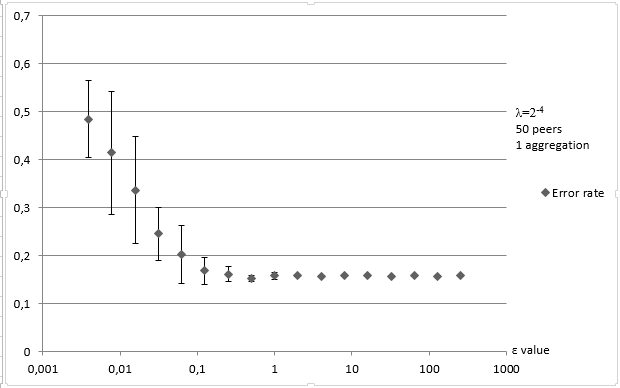
\includegraphics[width=\textwidth]{fig/spambase/epsilon_big_range}
	\caption{Effect of privacy level (Spambase)}
	\label{fig:epsilon_big_range}
\end{figure}

\subsubsection{Changes in $\lambda$}
\begin{figure}[H]
	\centering
	\begin{minipage}{.68\linewidth}
		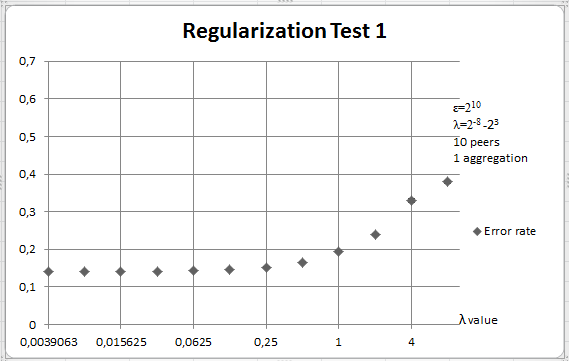
\includegraphics[width=\linewidth]{fig/spambase/regularization_extremelyhighepsilon}
		\captionof{figure}{Effect of regularization, no privacy (Spambase)}
		\label{fig:regularization_extremelyhighepsilon}
	\end{minipage}
	\hspace{1mm}
	\begin{minipage}{.68\linewidth}
		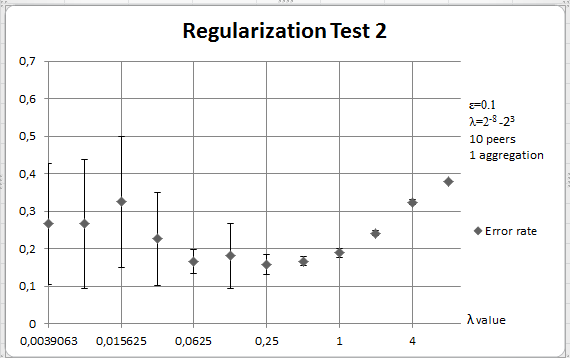
\includegraphics[width=\linewidth]{fig/spambase/regularization_normalepsilon}
		\captionof{figure}{Effect of regularization, common privacy (Spambase)}
		\label{fig:regularization_normalepsilon}
	\end{minipage}
	\hspace{1mm}
	\begin{minipage}{.68\linewidth}
		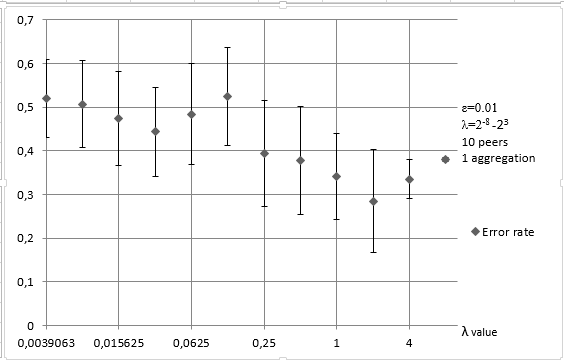
\includegraphics[width=\linewidth]{fig/spambase/regularization_lowepsilon}
		\captionof{figure}{Effect of regularization, high privacy (Spambase)}
		\label{fig:regularization_lowepsilon}
	\end{minipage}
\end{figure}


\subsection{Changes in data availability}
\begin{figure}[H]
	\centering
	\begin{minipage}{.65\linewidth}
		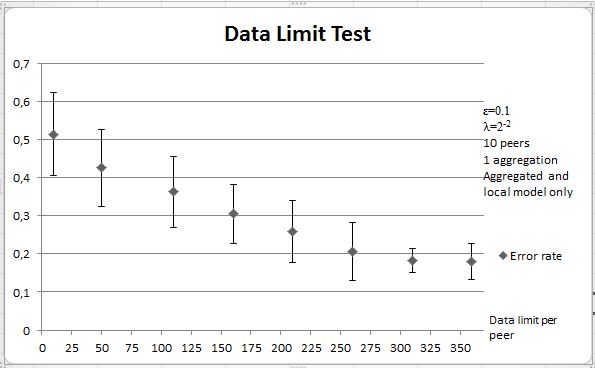
\includegraphics[width=\linewidth]{fig/spambase/data_limit_test_withoutlocalmodel}
		\captionof{figure}{$\epsilon = 0.1, \lambda = 2^{-2}$, 10 peers, 1 aggregations. Aggregated model only. (Spambase)}
		\label{fig:data_limit_test_withoutlocalmodel}
	\end{minipage}
	\hspace{1mm}
	\begin{minipage}{.65\linewidth}
		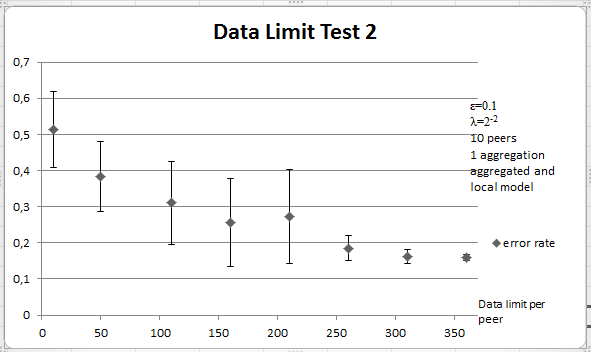
\includegraphics[width=\linewidth]{fig/spambase/data_limit_test_withlocalmodel}
		\captionof{figure}{$\epsilon = 0.1, \lambda = 2^{-2}$, 10 peers, 1 aggregation. Aggregated and local model. (Spambase)}
		\label{fig:data_limit_test_withlocalmodel}
	\end{minipage}
	\hspace{1mm}
	\begin{minipage}{.65\linewidth}
		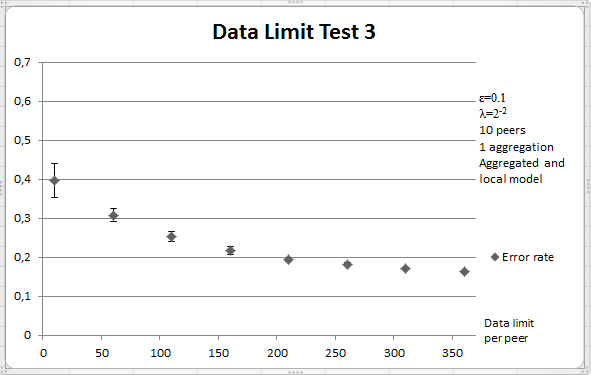
\includegraphics[width=\linewidth]{fig/spambase/data_limit_test_localmodelonly}
		\captionof{figure}{$\lambda = 2^{-2}$, 10 peers, local model only. (Spambase)}
		\label{fig:data_limit_test_localmodelonly}
	\end{minipage}
\end{figure}


\subsection{Changes in number of participants}
%\todo[inline]{make Effect of peer numbers into a simple table row showing min/max instead}
\begin{figure}[H]
	\centering
	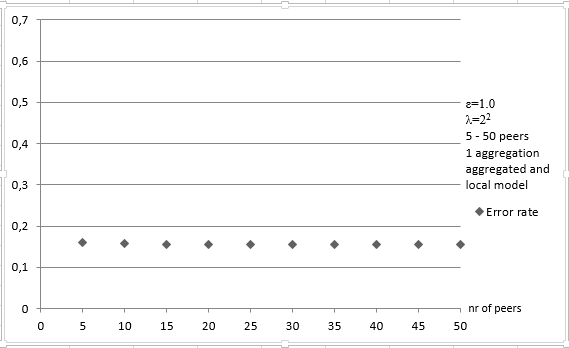
\includegraphics[width=\textwidth]{fig/adult/peer_range_constant_group}
	\caption{Effect of peer numbers. (Adult)}
	\label{fig:peer_range_constant_group}
\end{figure}


\subsection{Peer error rate variance}
\label{sec:results_peer_error_variance}
%\todo[inline]{replace variance table with numbers from recent, properly CVed runs. ALSO, add std.dev. of std dev. :)}
\begin{table}[H]
	\centering

	\begin{tabular}{|l|l|l|}
		\textbf{Model}                  & \textbf{Mean error} & \textbf{Peer std. dev.} \\
		\hline
		Local, no privacy      & 0,175 & 0.006 \\
		Aggregated, d. privacy & 0,158 & 0.000	 \\
		Ensemble with both & 0.166 & 0.002 \\
	\end{tabular}
	\caption{Variance among peers, (Adult)}
	\label{table:peer_variance_adult}
\end{table}      

\subsection{Effect of aggregation group size and model propagation}
\begin{table}[H]
	\centering
	\begin{tabular}{|l|l|l|l|}
		{\bf \begin{tabular}[c]{@{}l@{}}Group \\ size\end{tabular}} & {\bf \begin{tabular}[c]{@{}l@{}}Mean \\ error\end{tabular}} & {\bf \begin{tabular}[c]{@{}l@{}}Error\\ std. dev.\end{tabular}} & {\bf \begin{tabular}[c]{@{}l@{}}Peer error\\ std. dev.\end{tabular}} \\
		\hline
		1                                                           & 0.174                                                       & 0.0048                                                          & 0.0068                                                               \\
		5                                                           & 0.168                                                       & 0.0061                                                          & 0.0054                                                               \\
		10                                                          & 0.171                                                       & 0.0064                                                          & 0.0078                                                               \\
		15                                                          & 0.172                                                       & 0.0048                                                          & 0.0071                                                               \\
		20                                                          & 0.170                                                       & 0.0052                                                          & 0.0057                                                               \\
		25                                                          & 0.168                                                       & 0.0051                                                          & 0.0052                                                               \\
		30                                                          & 0.168                                                       & 0.0040                                                          & 0.0031                                                              
	\end{tabular}
	\caption{Effect of aggregation group size. Party-publishing. Adult.}
	\label{tab:results_groupsize_party}
\end{table}

\begin{table}[H]
	\centering
	\begin{tabular}{|l|l|l|l|}
		{\bf \begin{tabular}[c]{@{}l@{}}Group \\ size\end{tabular}} & {\bf \begin{tabular}[c]{@{}l@{}}Mean \\ error\end{tabular}} & {\bf \begin{tabular}[c]{@{}l@{}}Error \\ std. dev.\end{tabular}} & {\bf \begin{tabular}[c]{@{}l@{}}Peer error \\ std. dev.\end{tabular}} \\
		\hline
		1                                                           & 0.168                                                       & 0.0009                                                           & 0.0003                                                               \\
		5                                                           & 0.165                                                       & 0.0013                                                           & 0.0007                                                               \\
		10                                                          & 0.165                                                       & 0.0012                                                           & 0.0008                                                               \\
		15                                                          & 0.165                                                       & 0.0008                                                           & 0.0026                                                               \\
		20                                                          & 0.165                                                       & 0.0005                                                           & 0.0026                                                               \\
		25                                                          & 0.165                                                       & 0.0007                                                           & 0.0027                                                               \\
		30                                                          & 0.165                                                       & 0.0006                                                           & 0.0027                                                              
	\end{tabular}
	\caption{Effect of aggregation group size. All-publishing. Adult.}
	\label{tab:results_groupsize_all}
\end{table}

\subsection{Value of budgeting privacy}

\begin{figure}[H]
	\centering
	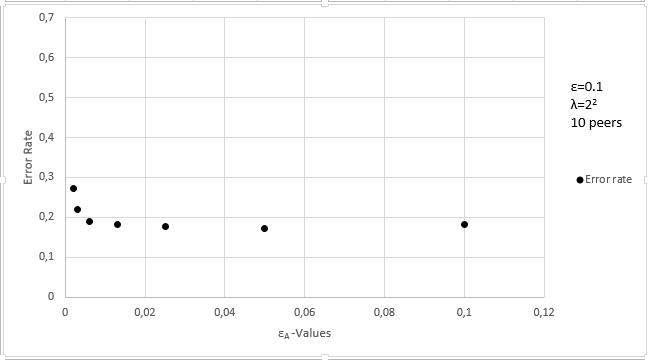
\includegraphics[width=.8\textwidth]{fig/adult/results_privacy_budget}
	\caption{Effect of Privacy Budgeting. (Adult)}
	\label{fig:results_privacy_budget}
\end{figure}


%add - some result showing what happens when the amount of privacy budget used is changed - possibly considering all vs party also here


\cleardoublepage